\cotefile{136}
\scanpage{252}
\diagram{\begin{tikzcd}[ampersand replacement=\&,column sep=large]
\mathcal N=\operatorname{Mod}(k) \arrow[r,"i",shift left] \& \mathcal M_0=\mathcal M^+ \arrow[l,"\unsure{\kappa|p}"',shift left]
\end{tikzcd}}
\diagram{\begin{tikzcd}[ampersand replacement=\&]
\deleted{\unsure{N|P|\mathcal N}}\arrow[r,sloped,allow upside down,"\deleted{/}" description] \& \deleted{\mathcal M_N}\& \deleted{\unsure{\mathcal M^+}}\\[-1ex]
\& \& |[draw,ellipse]|{i,p,\unsure{S|N|\mathcal N|\rho}}
\end{tikzcd}}
\[
\begin{aligned}
i(N)&=N\otimes_k S\\
\kappa(M_*)&=M_0
\end{aligned}
\]
\[
\tau_{N,0}\circ i:\mathcal N\longrightarrow\mathcal M_N
\]
a comme adjoint à droite,
\[
\kappa\circ\rho_{0N}=\kappa\circ\tau_0\circ\rho_N=\kappa\circ\rho_N
\]
\margin{\deleted{qui a comme adjoint à gauche}}

\uline{Conditions équivalentes}

a) $i_N=\tau_{N,0}\circ i$ est pl. fidèle

b) $\forall\,\deleted{\unsure{N}}P\in\operatorname{Mod}k,\quad
\deleted{\unsure{N}}P\xrightarrow{\sim}(\rho_N i_N(\deleted{\unsure{N}}P))_0$
\[
\left[\begin{aligned}
&=(\rho_N\tau_N(\deleted{\unsure{N}}P\otimes_k S))_0\\
&=(\rho_N(P\otimes_k\tau_N S))_0
\end{aligned}\right]
\]
c) $\kappa\circ\rho_N$ est un foncteur localisation

\figure{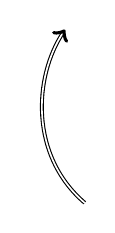
\begin{tikzpicture}[x=1cm,y=1cm]\draw[->,double] (0.4,0) .. controls (-0.3,0.6) and (-0.25,1.6) .. (0.15,2.2);\end{tikzpicture}}
\diagram{\begin{tikzcd}[ampersand replacement=\&]
\deleted{\unsure{\circ}} \& \deleted{M_0}\arrow[d] \& \deleted{M_1}\&\deleted{M_{\unsure{2|r}}\ \cdots}\\
\&\deleted{\unsure{P}}\&\&
\end{tikzcd}}
\deleted{$\unsure{\operatorname{Hom}_k(Q,P)}$}

\uline{Condition équivalente}

a$'$) \deleted{$\forall P\in\unsure{\operatorname{Mod}}$} $\operatorname{Im\,ess}i\subset\operatorname{Im\,ess}\rho_{0,N}$

b$'$) $\forall P\in\operatorname{Mod}k,$
\[
\begin{aligned}
i(P)&\xrightarrow{\sim}\rho_{0N}\tau_{N,0}\unsure{\circ i(P)|\circ(P)|i(P)}\\
&=\rho_{0N}i_N(P)
\end{aligned}
\]
b$'$\inserted{bis}) $\forall P\in\operatorname{Mod}k,\quad i(P)\xrightarrow{\unsure{\sim}}\rho_{0N}i_N(P)$ est un isom en dim $0\leq\alpha\leq N-1$

c$'$) \inserted{$\forall P\in\operatorname{Mod}k,$} $\forall\,0\leq\alpha\leq N-1,$ \deleted{$\tau_{N-\alpha,0}S$} on a
\diagram{\begin{tikzcd}[ampersand replacement=\&,row sep=small]
P\otimes_k S_\alpha \arrow[r,"\sim"] \& \operatorname{Hom}^{\alpha}(\tau_{N-\alpha}S,\deleted{\unsure{Q}}P\otimes_k S)\\
\bigl[\operatorname{Hom}^{\alpha}(S,P\otimes_k S)\bigr] \arrow[u,"\wr"'] \arrow[ur,dashed,"\text{\unsure{restrict.|restriction}}"' ] \&
\end{tikzcd}}
\[
\operatorname{Hom}^{\alpha}(S/\tau_{N-\alpha}S,P\otimes_k S)=0
\]
% archive sheet number: 251
